% !TeX spellcheck = en_AU-EnglishAustralia
% Preamble
\documentclass[12pt, a4paper]{article}
\usepackage[utf8]{inputenc}
%\usepackage[english]{babel}

\usepackage{indentfirst}
\usepackage{rotating, graphicx}
\usepackage{geometry}
\usepackage{hyperref}
\usepackage{amsmath}
\usepackage{amssymb}
\usepackage{gensymb}
\newgeometry{vmargin={30mm}}

\title{Speaker Research}	
\author{Laurence Prins}
\date{31.03.2021}
\usepackage[style=ieee]{biblatex}
\addbibresource{References.bib}

% Time total so far: 2.5 hours for researching basics, setting up document and starting math research
% Total time for audio physics research: 3 hours
% Time for audio calculations: .5 hours
% Total time learning how to reference and adding in sources: 2.5 hours
% Total Time for audio amplifiers: 3 hours
% Total time on speaker research: 2.5 + 3 + 2.5 + 3 = 11.5 hours

\begin{document}
	\maketitle
	\section{How does a speaker work}
	\subsection{The Basics}
	In the absolute basic sense, a speaker is an electromechanical system which converts electrical energy to mechanical energy (audio). \\
	
	The speaker consists of three major components, those being the magnet, the voice coil and the diaphragm. When current is passed through the voice coil an electric field is produced. This causes the voice coil, and all the components attached, to move away from the magnet\cite{howSpeaker}. Figure \ref{fig1:speakerexploded} shows this system. 
	
	The diaphragm, also called the cone, aims to perfectly mimic the behaviour of the voice coil. It converts the mechanical motion of the voice coil into acoustic energy, thus the material of the diaphragm will affect the response of the speaker. The common material of choice is paper, plastic or metal\cite{speakerDiaphragm}.
	
	\begin{figure}[!htb]
		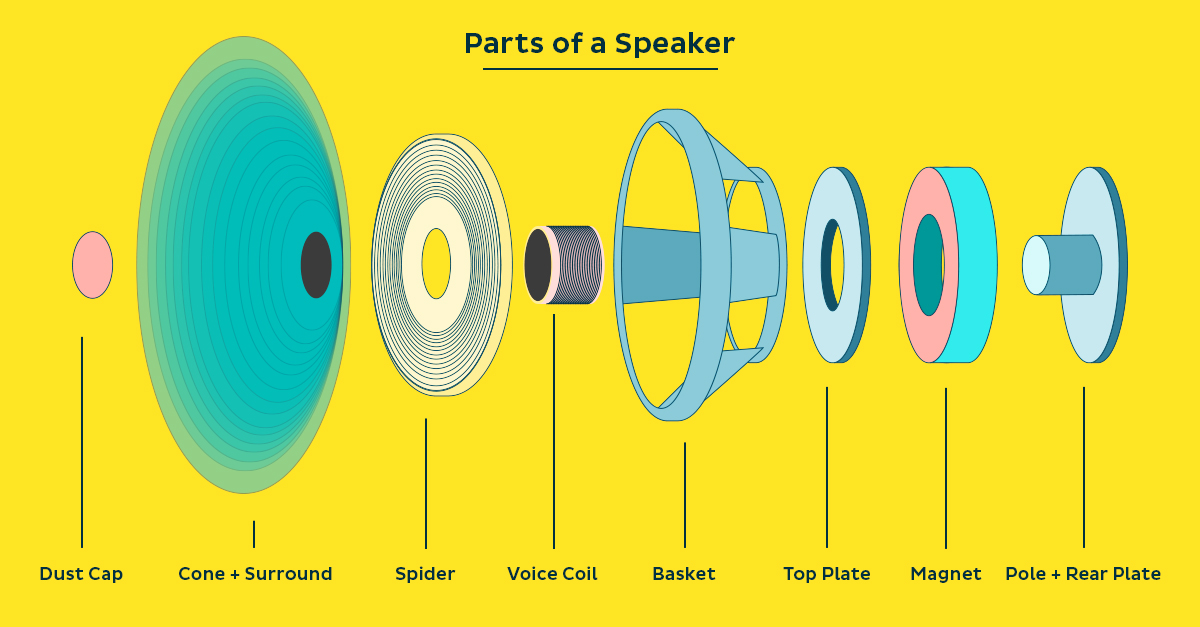
\includegraphics[width=\textwidth]{./Figures/parts_of_a_speaker}
		\caption{Parts of a speaker, source: \cite{howSpeaker}}
		\label{fig1:speakerexploded}
	\end{figure}
	Speakers have different frequency responses which tell how well the speaker will work at various frequencies. The goal is to get a flat frequency response, meaning the speaker will have the same response for all frequencies. Tweeters are speakers which are designed to produce high frequency audio (~2kHz – 20kHz), they are often smaller than woofers. Woofers are designed to produce low frequency audio (50Hz – 1kHz) and are generally larger speakers \cite{speakerTypes}.

	\section{Speaker Maximums}
	\subsection{Frequency Response}
		- Increasing frequency response
	- Add more speakers like in \cite{howSpeaker}
	- Equaliser
	\subsection{Waveforms}
	- What waveforms will break the speaker over time.		
	\section{Speaker Simulation}
	- How to model the speaker - Equivalent circuit
	- Treat speaker as a BPF?
	\section{Sound Parameters}
	%==================================================================================%
	%-================================--Sound Power--=================================-%
	%==================================================================================%
	\subsection{Sound Power (SWL)}
	Sound power is the rate at which sound energy is emitted. The sound power of a speaker is generally given in decibels (dB). The formula for calculating the power in decibels is given in equation \ref{eqn:SWL}. \cite{audioParameters}\cite{soundPower}
	\begin{equation}
		\label{eqn:SWL}
		L_W = 10log\left(\frac{P}{P_0}\right)
	\end{equation}
	\begin{center}
		\textit{Where P is the sound power of the speaker, $P_0$ is the reference sound power and $L_W$ is Sound Power Level (SWL). The reference sound power is set to $10^{-12}$ W, which is the lowest power sound a person could theoretically hear (i.e. someone with perfect hearing)}. 	 %http://www.sengpielaudio.com/calculator-soundpower.htm
	\end{center}
	%==================================================================================%
	%-===============================--Sound Intensity--==============================-%
	%==================================================================================%
	\subsection{Sound Intensity (SIL)}
	Sound intensity is the measure of sound power per unit area. It is related to sound power by the formula in equation \ref{eqn:soundIntensityGeneralForm}\cite{soundIntensity}
	\begin{equation}
		\label{eqn:soundIntensityGeneralForm}
		I(r) = \frac{P}{A(r)}
	\end{equation}
	\begin{center}
		\textit{where P is the sound power at the source (W) and A(r) is the area as a function of distance from the source.}
	\end{center}
	For example, a spherical sound source will have a sound intensity which varies with distance at a rate shown in equation \ref{eqn:soundIntensitySphere}.
	\begin{equation}	
		\label{eqn:soundIntensitySphere}
		I = \frac{P}{4\pi r^2}
	\end{equation}
	This is the inverse square law and it states that the sound intensity is proportional to the inverse of the distance from the source. i.e.
	\begin{equation*}
		I \propto \frac{1}{r^2}
	\end{equation*}
	
	Speakers will produce a spherical sound wave in the direction of the source and therefore can be treated as a point source in a spherical field. Sound power is constant, therefore using the inverse square law the intensity at any distance can be calculated using the formula in equation \ref{eqn:soundIntensityDistanceProperty}. \cite{audioParameters} 
	
	\begin{equation}	
		\begin{aligned}
		\label{eqn:soundIntensityDistanceProperty}
		I_1r_1^2 = I_2r_2^2 \\
		\implies \frac{I_1}{r_2^2} = \frac{I_2}{r_1^2}
		\end{aligned}
	\end{equation}
	
	Sound intensity is often given in decibels, this is calculated using equation \ref{eqn:SIL}.
	\begin{equation}
		\label{eqn:SIL}
		L_I = 10log\left(\frac{I}{I_0}\right)
	\end{equation}
	\begin{center}
		\textit{Where $L_I$ is the Sound Intensity Level (SIL) and $I_0$ is the intensity threshold of hearing, $10^{-12}$ $W/m^2$} 
	\end{center}
	%==================================================================================%
	%-===============================--Sound Pressure--===============================-%
	%==================================================================================%
	\subsection{Sound Pressure (SPL)}
	Sound pressure is the average variation in atmospheric pressure caused by sound. Sound pressure is often given in dB, calculated through equation \ref{eqn:SPL}. \cite{soundPressure}
	\begin{equation}
		\label{eqn:SPL}
		L_P = 20log\left(\frac{P}{P_0}\right)
	\end{equation}
	\begin{center}
		\textit{Where $L_P$ is the Sound Pressure Level (SPL), P is the rms sound pressure in Pa and $P_0$ is the reference sound pressure equal to $2x10^{-5}Pa$ which is the threshold of human hearing}
	\end{center}
	Sound pressure is related to sound intensity through equation \ref{eqn:intensityPressureRelationship}.
	\begin{equation}
		\label{eqn:intensityPressureRelationship}
		I = pv
	\end{equation}
	\begin{center}
		\textit{where p is sound pressure and v is the particle velocity, both are functions of distance from the source}
	\end{center}
	The sound pressure at two points can be related based on the equations in \ref{eqn:intensityPressureRelationship} and \ref{eqn:soundIntensityDistanceProperty} results in equation \ref{eqn:soundPressureDistanceRelation}. 
	\begin{equation}
		\label{eqn:soundPressureDistanceRelation}
		p_2 = \frac{r_1}{r_2}p_1
	\end{equation}
	\begin{center}
		\textit{where $p_n$ is the pressure at point n in Pa, $r_n$ is the distance from the source in m}
	\end{center}
	Sound pressure and sound power can be related through equation \ref{eqn:soundPowerPressureRelation}. \cite{soundPowerCalculator}
	\begin{equation}
		\label{eqn:soundPowerPressureRelation}
		L_W = L_P + 10log\left(\frac{A_s}{A_0}\right)
	\end{equation}
	\begin{center}
		\textit{where $A_s$ is an area of a surface which fully encompasses the source and $A_0$ = 1$m^2$}
	\end{center}
	For certain areas drawn around the source, this can be simplified into equation \ref{eqn:soundPowerPressureRelation2} \cite{soundPower}
	\begin{equation}
		\label{eqn:soundPowerPressureRelation2}
		\begin{aligned}
			\textbf{Sphere:}		L_W = L_P + 20log(r) + 11 dB \\
			\textbf{Hemishpere:}    L_W = L_P + 20log(r) + 8dB 
		\end{aligned}
	\end{equation}
	%==================================================================================%
	%-================================--Our Speaker--=================================-%
	%==================================================================================%
	\pagebreak
	\section{Our Speaker}
	%==================================================================================%
	%-===============================--Specifications--===============================-%
	%==================================================================================%
	\subsection{Specifications}
	
	We have an AS01508MS-SP11-WP-R speaker with the specifications shown in \ref{tab:speakerSpecs}.\\
	The frequency response shown in \ref{fig:speakerFreq}. The speaker has the best output between 600Hz and 20kHz. Between these frequencies the average sensitivity is 89dB SPL or 0.564Pa of sound pressure at 10cm away from the speaker. 
	
	\begin{table}[!htb]
		\caption{Specifications for AS01508MS-SP11-WP-R speaker, source: \cite{speakerDatasheet}}
		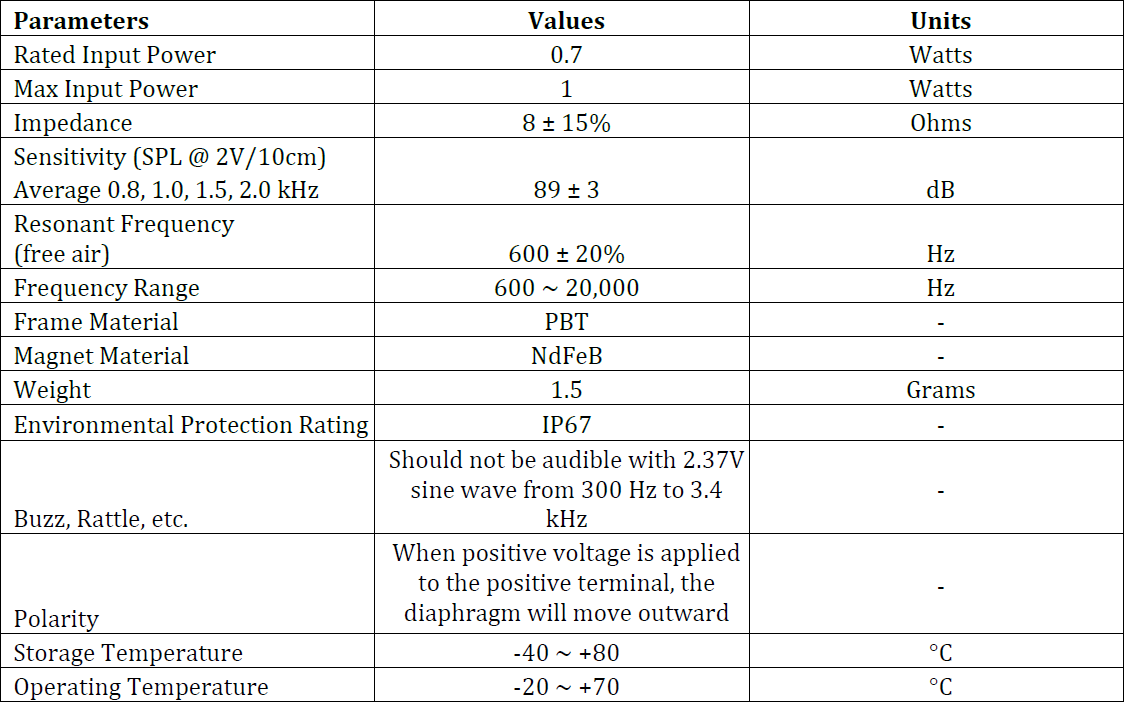
\includegraphics[width=\textwidth]{./Figures/speaker_specifications}
		\label{tab:speakerSpecs} 
	\end{table} 
	
	\begin{figure}[!htb]
		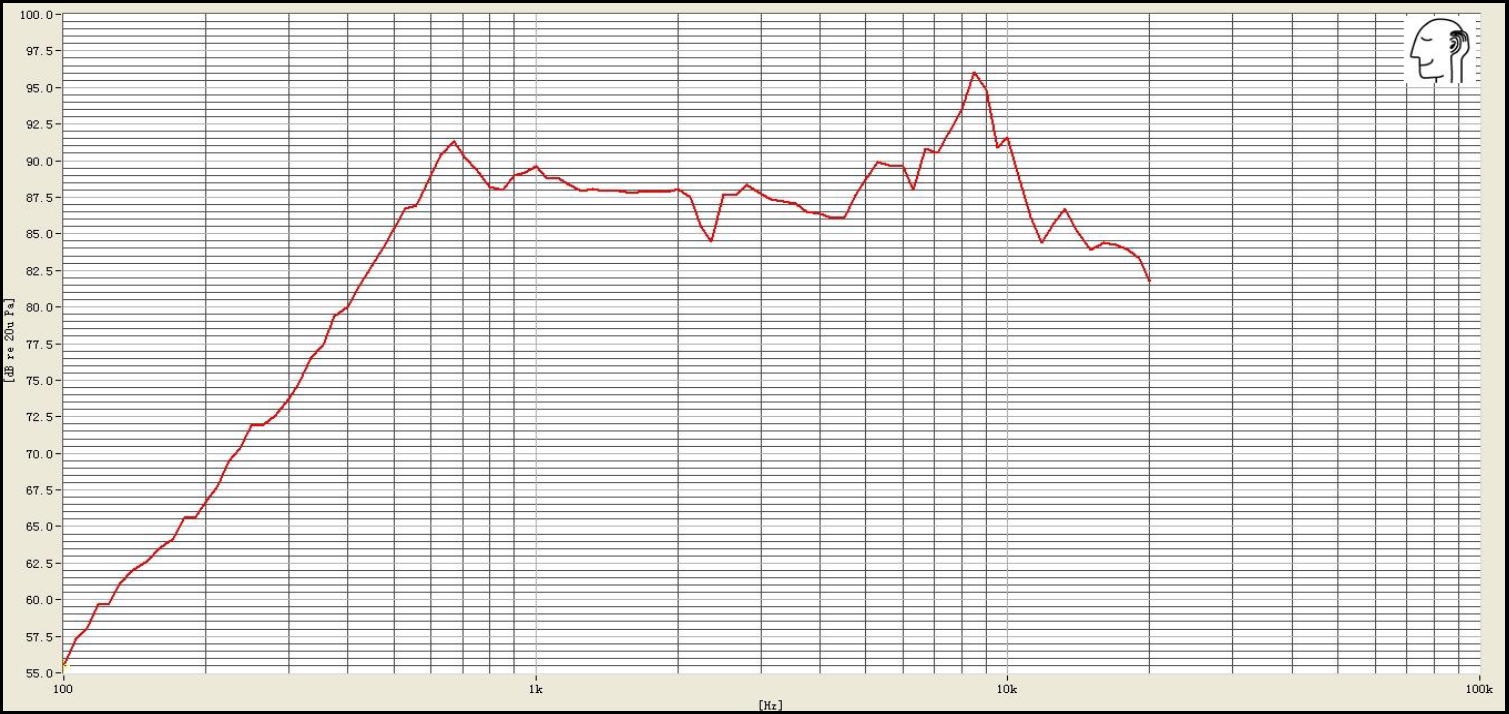
\includegraphics[width=\textwidth]{./Figures/speaker_freq_response}
		\caption{Frequency response for AS01508MS-SP11-WP-R speaker, source: \cite{speakerDatasheet}}
		\label{fig:speakerFreq}
	\end{figure}
	%==================================================================================%
	%-===============================--Speaker Power--================================-%
	%==================================================================================%
	\pagebreak
	\subsection{Speaker Power and Efficiency} 
	Following the calculation in \cite{soundPowerCalculator} and equation \ref{eqn:soundPowerPressureRelation}. The sound pressure measurement was done with the speaker attached to a baffle board with the microphone at 10cm or 0.1m away. From figure \ref{fig:speakerDims}, the radius between the centre of the speaker and the hemisphere must be 0.1 + (1/2)(0.0035)m = 0.102m. The area of the hemisphere is thus:
	\begin{equation*}
		A = 2 \pi r^2 = 2\times\pi\times0.102^2 = 0.065m^2
	\end{equation*}
	Using the average 89dB output, the sound power estimate is then calculated:
	\begin{equation}
		L_W = L_P + 10log\left(\frac{A}{A_0}\right) \therefore L_W = 89\pm3 + 10log\left(0.065\right) = 77.2dB \pm 3
		\label{eqn:ourSpeakerPower}
	\end{equation}
	Alternatively, following equation \ref{eqn:soundPowerPressureRelation2} results in:
	\begin{equation*}
		L_W = L_P + 20log(0.102) + 8 dB = 77.2dB\pm3
	\end{equation*}
	\begin{figure}[!htb]
		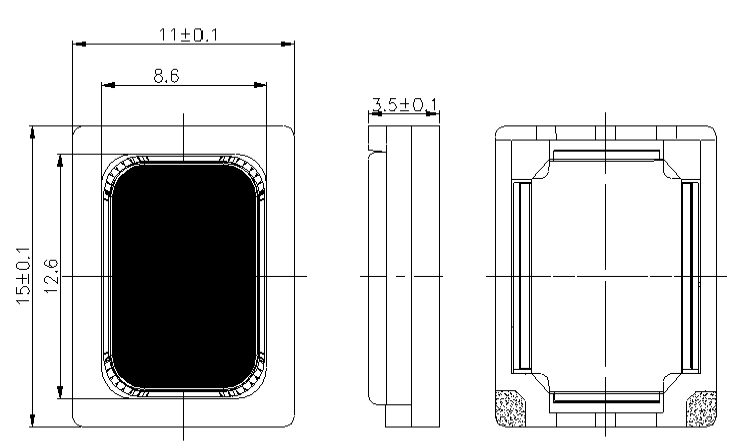
\includegraphics[width=\textwidth]{./Figures/speaker_dimensions}
		\caption{Dimensions of AS01508MS-SP11-WP-R speaker, source:\cite{speakerDatasheet}}
		\label{fig:speakerDims}
	\end{figure}

	This result is useful as it can be used on the simulator \url{https://noisetools.net/noisecalculator2}.\\
	
	The speaker efficiency can be calculated using the result from \ref{eqn:ourSpeakerPower}. From equation \ref{eqn:SWL} the output sound power is P = 52.4$\mu$W. With an input of 0.5W, the efficiency is:
	\begin{equation*}
		\eta = \frac{52.4\mu}{0.5}\times 100\% = 1.05\%
	\end{equation*}
	
	%==================================================================================%
	%-===============================--Speaker Maximum--==============================-%
	%==================================================================================%
	\pagebreak
	\subsection{Speaker Maximum}
	Our speaker has an output of 89dB SPL at 10cm with a 2V input at 1kHz. The speaker has 8$\Omega$ impedance thus the power input per output is:
	\begin{equation}
		P = \frac{V^2}{R} = \frac{2^2}{8} = 0.5W
	\end{equation}
	Note: This is only true for some frequencies. The speaker has a maximum impedance of 11.4$\Omega$ at 600 Hz and 20kHz.  
	From table \ref{tab:speakerSpecs}, the speaker is rated for 0.7W and has a maximum input power of 1. This means we can double the power input. Based on the 3dB rule, this will only result in a 3dB increase in audio pressure\cite{speakerPowerDistance}. Thus the average maximum output from the speaker will be:
	\begin{center}
		92 $\pm$ 3dB at 1W input power
	\end{center}
	This is the maximum and running the speaker at above this input power for a period could result in damage done to the device. 
	%==================================================================================%
	%-=============================--Speaker Drive Circut--===========================-%
	%==================================================================================%
	\pagebreak
	\section{Speaker Amplifiers}

	\subsection{Introduction}
	Speakers typically require more power input than the output from a microcontroller pin can provide. Therefore we need a drive circuit to control the speaker. Our speaker is rated for 0.7W with a maximum of 1W input. Any less input will result in a lower than expected power output and any higher will burn out the voice coil and kill the speaker. There are various classes of amplifiers, the class is defined based on how much of the waveform does the active device conduct.
	\subsection{Class A Amplifier}
	In a class A amplifier, the output device conducts through the full waveform (360\degree). The most simple way to drive the speaker is to drive a BJT to control the input to the speaker this is shown in figure \ref{fig:speakerDriver1} (left). The circuit shown in figure \ref{fig:speakerDriver1} (right) shows a more complex class A amplifier which includes biasing and coupling and bypass capacitors to make a more reliable output. To operate for the full waveform, the transistor needs to be correctly biased such that it operates within its linear region.
	
	\begin{figure} [!htb]
		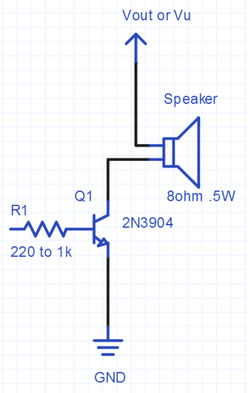
\includegraphics[width=50mm, scale=0.4]{./Figures/Speaker_Driver_1}
		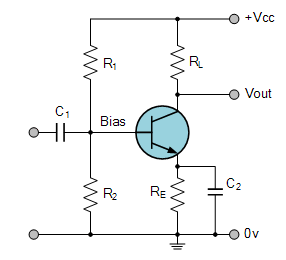
\includegraphics[scale = 1.0]{./Figures/class_A_amplifier_biasing}
		\caption{\textbf{Left:} simple speaker drive circuit. Source: \cite{speakerDriveSimple} \textbf{Right:} Class A amplifier circuit. Source: \cite{amplifiers}}.
		\label{fig:speakerDriver1}
	\end{figure}

	\textbf{Advantages}
	\begin{itemize}
		\item Simple, only has one active component therefore could easily be built without the need of a separate IC
		\item Low levels of distortion implies a high fidelity output
	\end{itemize}
	\textbf{Disadvantages}
	\begin{itemize}
		\item Inefficient, constant operation of the BJT in the active region causes power loss meaning the maximum theoretical efficiency is around 30\% 
		\item Need to correctly bias the transistor base DC voltage to allow for correct operation and low distortion
		\item Power supply must be sized correctly due to high idle current from the amplifier
	\end{itemize}
	% ====================== Class B amplifiers	==============================
	\subsection{Class B Amplifier "Push Pull"}
	Can improve on the efficiency of the class A amplifier by adding a complimentary pnp BJT. Class B amplifiers are defined based on each active component operating for half of the waveform (180\degree).  An example of a class B amplifier is given in figure \ref{fig:classBAmplifier} which also shows decoupling capacitors and resistors for correctly biasing the transistors. The npn transistor conducts for the positive half of the cycle and the pnp transistor conducts for the negative half of the waveform. At the zero-crossing point of the waveform, neither of the transistors will conduct and thus will end up having a deadzone causing distortion in the output waveform. 
	\begin{figure} [!htb]
		\hfill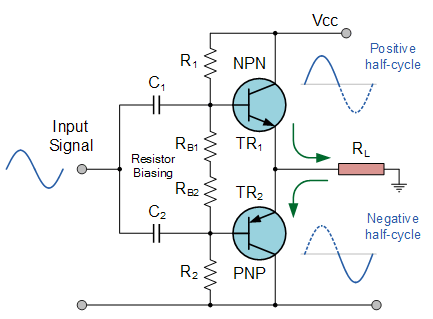
\includegraphics{./Figures/class_B_amplifier_biasing}\hspace*{\fill}	
		\caption{Class B amplifier circuit, source: \cite{amplifiers}}
		\label{fig:classBAmplifier}
	\end{figure}

	\textbf{Advantages}
	\begin{itemize}
		\item More efficient than class A amplifier as each transistor operates 50\% of the time. Theoretical maximum efficiency is 78.5\%.
		\item Operating point of transistors is at around 0V
		\item Low standing bias (no input) current and thus low power consumption with no signal
	\end{itemize}

	\textbf{Disadvantages}
	\begin{itemize}
		\item The distortion at the crossover point makes the amplifier not useful for audio amplifier application
		\item More distortion than a class A amplifier

	\end{itemize}
	Since we care about the zero-crossing point of the waveform for distance measurements, this class of amplifier is unfit for our use. 
	% ========================= Class AB Amplifiers	=============================
	\pagebreak
	\subsection{Class AB Amplifier}
	Uses diodes, each transistor now conducts partially during the other transistors region. This reduces the distortion at the crossover point. Class AB each active component operates for between half the wave and the full wave (180\degree - 360\degree) depending on the biasing of the diodes. An example of a class AB amplifier is given in figure \ref{fig:classABAmplifier}.\\
	\begin{figure} [!htb]
		\hfill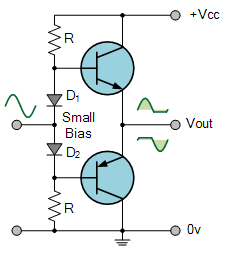
\includegraphics{./Figures/class_AB_amplifier}\hspace*{\fill}	
		\caption{Class AB amplifier circuit, source: \cite{amplifiers}}
		\label{fig:classABAmplifier}
	\end{figure}
	
	\textbf{Advantages}
	\begin{itemize}
		\item Can be more efficient than a class A amplifier if biased correctly
		\item Eliminates the distortion at the crossover point with class B therefore higher fidelity output signal
		
	\end{itemize}
	
	\textbf{Disadvantages}
	\begin{itemize}
		\item Less efficient than a class B amplifier, depends on biasing set by the diodes
		\item More complicated, have to correctly bias
	\end{itemize}
	% ========================	Class D Amplifiers ===============================
	\pagebreak
	\subsection{Class D Amplifier}
	Class D amplifiers use PWM to control the amplifier. The block diagram for this class of amplifier is given in figure \ref{fig:classDAmplifier} and an example of the circuit is given in figure \ref{fig:classDAmplifierCircuit}. Here the inductors and capacitors form a low-pass filter which takes the PWM input and forms the amplified sine wave which is fed to the speaker. Each output transistor is on and passes its full current when conducting, therefore there is very little voltage drop and thus power loss across the transistors. Class D amplifiers are a class of switching amplifiers, the active components act as switches as opposed to linear gain devices like in class A, B and AB above.
	\begin{figure} [!htb]
		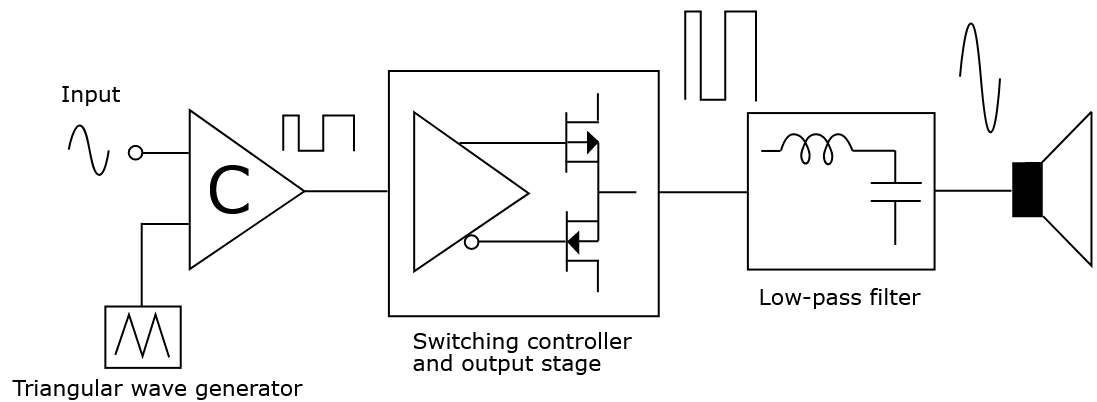
\includegraphics[scale=0.5]{./Figures/class_D_amplifier}
		\caption{Class D amplifier block diagram, source: \cite{classDamplifiercircuit}.}
		\label{fig:classDAmplifier}
	\end{figure}
	\begin{figure} [!htb]
		\hfill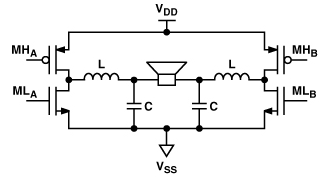
\includegraphics{./Figures/class_D_amplifier2}\hspace*{\fill}	
		\caption{Class D amplifier circuit, source: \cite{classDamplifier}}
		\label{fig:classDAmplifierCircuit}
	\end{figure}
	
	\textbf{Advantages}
	\begin{itemize}
		\item Can reach up to 90\% efficiency, on paper can reach 100\%
		\item No need for biasing circuitry therefore less loss from biasing components
	\end{itemize}
	
	\textbf{Disadvantages}
	\begin{itemize}
		\item More active components than the other circuits
	\end{itemize}
	
	\pagebreak
	\subsection{Chosen Amplifier}
	
	\subsection*{Notes}
	 - Speaker moves both ways therefore want to have the resting position at 0V in order to be more efficient. \\
	 - Need to bias transistors such that the input voltage should exceed cut in voltage. BJT needs to be in the active region to operate as an amplifier. \url{https://www.tutorialspoint.com/amplifiers/transistor_biasing.htm}
	 - Useful for calculating values for biasing: \cite{classAbiasing}
	
	\printbibliography[title={References}]
		
\end{document}
